\section{Постановка задачи}

Цель работы --- освоить синтез изображений трёхмерной сцены методом обратной
трассировки путей и проверить корректность расчёта освещения. Требуется построить
изображение треугольной сцены из точечной камеры, учесть локальное освещение и
тени, а затем преобразовать абсолютные значения яркости в восьмибитное
изображение. Параметры сцены должны задаваться так, чтобы при их изменении
можно было повторить расчёт.

\section{Параметры сцены}

Сцена представляет собой комнату размером \(3{,}3\times3{,}3\times3{,}3\) м с
открытой передней стороной. Ось \(y\) направлена вверх, камера расположена со
стороны положительных \(z\). Из 34 треугольников 10 составляют стены, пол и потолок,
а 24 образуют два повёрнутых параллелепипеда. Высокий матовый параллелепипед
расположен слева, низкий глянцевый --- справа. Боковые стены имеют разные
коэффициенты отражения, поэтому по цвету их вкладов можно наблюдать перенос
света между поверхностями.

\begin{table}[ht]
\centering
\caption{Геометрические параметры объектов}
\begin{tabular}{lccc}
\toprule
Объект & Центр \((x;y;z)\), м & Размер вдоль осей, м & Поворот вокруг \(y\) \\
\midrule
Матовый & \((-0{,}68;0{,}90;-0{,}55)\)
 & \(0{,}94\times1{,}80\times0{,}92\) & \(-19^\circ\) \\
Глянцевый & \((0{,}64;0{,}42;0{,}39)\)
 & \(1{,}02\times0{,}84\times1{,}02\) & \(25^\circ\) \\
\bottomrule
\end{tabular}
\end{table}

Камера установлена в точке \((0;1{,}65;5{,}85)\) м, направлена на точку
\((0;1{,}65;0)\) м и имеет вертикальный угол обзора \(42^\circ\). Тёплый
источник освещает сцену спереди, холодный расположен ближе к задней стене.
Указанные в таблице векторы осей нормируются перед расчётом. Три канала линейной
модели RGB представляют три условные полосы излучения, рассчитываемые
независимо. Все материалы непрозрачны.

\begin{table}[ht]
\centering
\caption{Параметры точечных источников}
\begin{tabular}{lccc}
\toprule
Источник & Положение, м & Вектор оси & \(I_0\), Вт/ср по каналам \\
\midrule
Тёплый & \((-0{,}72;3{,}05;1{,}08)\) & \((0{,}16;-1;-0{,}34)\) & \((32;27;20)\) \\
Холодный & \((1{,}08;2{,}72;-0{,}92)\) & \((-0{,}12;-1;0{,}19)\) & \((10;12;18)\) \\
\bottomrule
\end{tabular}
\end{table}

\begin{table}[ht]
\centering
\caption{Коэффициенты диффузного отражения}
\begin{tabular}{lc}
\toprule
Поверхность & \(K_d=(R;G;B)\) \\
\midrule
Пол, потолок и задняя стена & \((0{,}76;0{,}71;0{,}62)\) \\
Левая стена & \((0{,}68;0{,}10;0{,}048)\) \\
Правая стена & \((0{,}16;0{,}49;0{,}26)\) \\
Матовый параллелепипед & \((0{,}72;0{,}51;0{,}28)\) \\
Глянцевый параллелепипед & \((0{,}035;0{,}16;0{,}21)\) \\
\bottomrule
\end{tabular}
\end{table}

\clearpage
\section{Пересечение лучей и локальное освещение}

Для каждой случайной точки пикселя строится луч \(x(t)=o+t\omega\), где \(o\) ---
положение камеры, а \(\omega\) --- единичное направление через плоскость экрана.
Для треугольника с вершинами \(a,b,c\) вычисляется пересечение с его плоскостью
\[
 t=\frac{(a-o)\cdot n}{\omega\cdot n},
 \qquad x(t)=a+u(b-a)+v(c-a).
\]
Среди пересечений с \(t>0\), \(u\ge0\), \(v\ge0\) и \(u+v\le1\) выбирается
ближайшее. Нормаль поверхности ориентируется к предыдущей точке пути.

Пусть \(y_j\) --- положение источника, \(H_j\) --- его единичная ось,
\(\omega_i=(y_j-x)/R\), \(R=\lVert y_j-x\rVert\), а
\(\omega_o\) --- направление к предыдущей точке пути. При обозначении
\(\pos{a}=\max(a,0)\) интенсивность и освещённость имеют вид
\[
 I_j(-\omega_i)=I_{0,j}\pos{-\omega_i\cdot H_j},\qquad
 E_j(x)=\frac{I_j(-\omega_i)}{R^2}\pos{n\cdot\omega_i}.
\]
Коэффициент видимости \(v(x,y_j)\) равен нулю, если теневой луч пересекает
треугольник до источника, и единице в остальных случаях. Начало теневого
луча и луча продолжения смещается на \(10^{-6}\) м вдоль нормали, чтобы
исключить самопересечение.

Ламбертовской яркости \(L=K_dE/\pi\) соответствует ДФО \(K_d/\pi\).
Для глянцевого объекта к ней добавляется составляющая Кука--Торранса.
При \(c_i=n\cdot\omega_i>0\) и \(c_o=n\cdot\omega_o>0\) модель имеет вид
\[
 f_r(x,\omega_i,\omega_o)=\frac{K_d}{\pi}
  +K_s\frac{D(h)G(\omega_i,\omega_o)F_r(\omega_o)}{4c_i c_o},
 \qquad h=\frac{\omega_i+\omega_o}{\lVert\omega_i+\omega_o\rVert}.
\]
Здесь \(K_d\) и \(K_s\) --- поканальные коэффициенты материала. Для
глянцевого параллелепипеда \(K_d=(0{,}035;0{,}16;0{,}21)\),
\(K_s=(0{,}92;0{,}80;0{,}74)\). Для матовых материалов \(K_s=0\).
При неположительном \(c_i\) или \(c_o\) значение ДФО равно нулю.

Плотность нормалей микрограней задана распределением Бекмана с параметром
шероховатости \(\alpha=0{,}32\). Положим \(c_h=n\cdot h\) и \(q=\omega_o\cdot h\).
Тогда плотность и геометрический множитель имеют вид
\[
 D(h)=\frac{\exp\!\bigl(-(1-c_h^2)/(\alpha^2c_h^2)\bigr)}
                 {\pi\alpha^2c_h^4},\qquad
 G(\omega_i,\omega_o)=\min\left(1,\frac{2c_hc_i}{q},\frac{2c_hc_o}{q}\right).
\]
Для неполяризованного света \(F_r=(R_s+R_p)/2\). При переходе из воздуха к
микрограни с показателем преломления \(n_2=1{,}55\) закон Снеллиуса даёт
\(c_t=\sqrt{1-(1-q^2)/n_2^2}\). Коэффициенты отражения по энергии равны
\[
 R_s=\left(\frac{q-n_2c_t}{q+n_2c_t}\right)^2,\qquad
 R_p=\left(\frac{c_t-n_2q}{c_t+n_2q}\right)^2.
\]
Показатель преломления здесь используется для расчёта отражения от
микрограней. Свет внутри объектов не трассируется.

\clearpage
\section{Обратная трассировка путей}

Пути начинаются в камере. При каждом попадании в поверхность выполняется
оценка следующего события. Для этого из точки \(x\) строится теневой луч к
каждому точечному источнику, а яркость прямого освещения определяется суммой
\[
 L_d(x,\omega_o)=\sum_j v(x,y_j)\,E_j(x)\,f_r(x,\omega_{i,j},\omega_o).
\]
Поскольку источников два, сумма вычисляется полностью. Косинус приёмника
входит в \(E_j\) один раз. Яркость в направлениях, покидающих сцену, равна
нулю.

Для оценки вторичного освещения следующий луч выбирается в полусфере
относительно \(n\). При независимых \(u_1,u_2\sim U[0,1)\) его координаты в
локальном ортонормированном базисе равны
\[
 \omega_i'=\left(\sqrt{u_1}\cos(2\pi u_2),
                 \sqrt{u_1}\sin(2\pi u_2),\sqrt{1-u_1}\right),\qquad
 p(\omega_i)=\frac{n\cdot\omega_i}{\pi}.
\]
Вклад прямого освещения в каждом узле умножается на накопленный вес
\(\beta_i\). При переходе к следующей поверхности вес изменяется по формуле
\[
 \beta_0=1,\qquad
 \beta_{i+1}
 =\beta_i\frac{f_r(x_i,\omega_i,\omega_o)(n\cdot\omega_i)}{p(\omega_i)}
 =\beta_i\,\pi f_r(x_i,\omega_i,\omega_o).
\]
У ламбертовского материала множитель сокращается до \(K_d\).
Яркость одного пути с \(m\) попаданиями равна
\(\sum_{i=0}^{m-1}\beta_i L_d(x_i,\omega_o)\). В расчёте учитывается до
четырёх попаданий. Ограничение глубины отсекает вклад путей более высокого
порядка.

\section{Формирование изображения}

Разрешение составляет \(500\times500\) пикселей. Каждый пиксель делится на
сетку \(6\times6\). В каждой ячейке выбирается одна случайная точка,
поэтому яркость пикселя равна среднему по 36 путям. Такая стратификация
сглаживает границы треугольников и теней. Начальное состояние генератора
фиксировано числом 5.

Прямой вклад первого попадания и сумму вторичных вкладов программа
сохраняет в абсолютных единицах по каждому каналу. Для восьмибитных
изображений используется общий уровень белого \(L_{\mathrm{white}}=4\,
\radiance\) на канал. Если \(L_c\) --- яркость канала, то код пикселя равен
\[
 V_c=\operatorname{round}\!\left[
  255\left(\min\!\left(1,\max\!\left(0,\frac{L_c}{L_{\mathrm{white}}}\right)\right)
         \right)^{1/2{,}2}\right].
\]
Так можно сравнить два изображения при одинаковой экспозиции.

Геометрия, камера, материалы и источники задаются в файле сцены JSON.
Через командную строку выбираются файл сцены, разрешение, число путей
на пиксель, предельная глубина и уровень белого.

\clearpage
\section{Результаты}

\begin{figure}[ht]
\centering
\begin{minipage}[t]{0.48\textwidth}
\centering
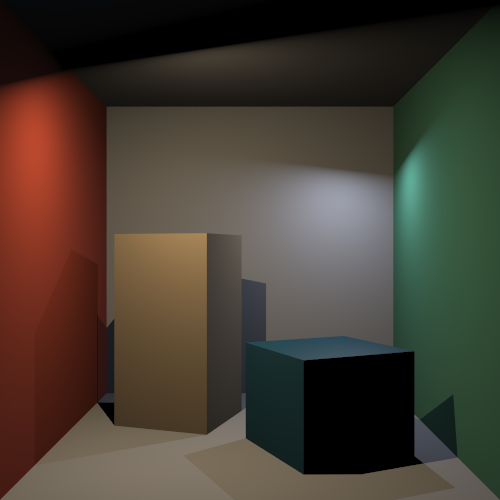
\includegraphics[width=\linewidth]{direct.png}\par
\small а) Прямое освещение
\end{minipage}
\hfill
\begin{minipage}[t]{0.48\textwidth}
\centering
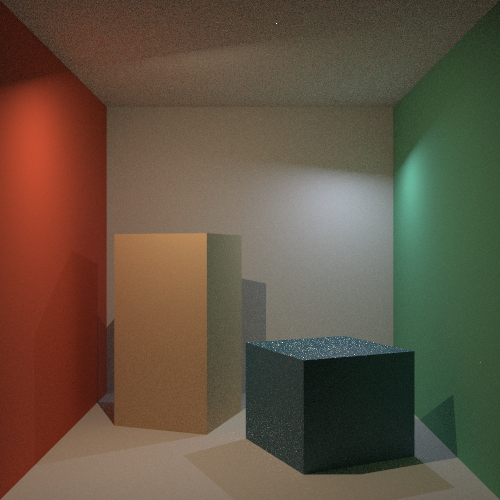
\includegraphics[width=\linewidth]{render.png}\par
\small б) Прямое и вторичное освещение
\end{minipage}
\caption{Изображения сцены при одинаковой экспозиции}
\label{fig:scene}
\end{figure}

На рис.~\ref{fig:scene},~а видны границы теней от двух точечных источников.
На переднюю грань глянцевого параллелепипеда прямой свет не попадает.
После добавления вторичного освещения различимы эта грань и потолок.
На потолке слева заметен тёплый оттенок, обусловленный отражением от
терракотовой стены. На верхней грани глянцевого объекта видны
квазизеркальные отражения. Остаточное зерно на изображении связано с
конечным числом случайных путей и особенно заметно в этой области.

\begin{table}[ht]
\centering
\caption{Средняя абсолютная яркость по кадру, \(\radiance\) на канал}
\begin{tabular}{lccc}
\toprule
Вклад & \(R\) & \(G\) & \(B\) \\
\midrule
Прямой & 0,35133 & 0,26140 & 0,19288 \\
Вторичный & 0,23269 & 0,14532 & 0,07623 \\
Суммарный & 0,58403 & 0,40673 & 0,26912 \\
\bottomrule
\end{tabular}
\end{table}

На участке передней грани глянцевого объекта (столбцы 340--379 и строки
386--413, отсчёт от нуля из верхнего левого угла) средний прямой вклад
равен нулю по всем каналам. Средний вторичный вклад на этом участке
составил \((0{,}01320;0{,}03900;0{,}02593)\,\radiance\).
При преобразовании полного изображения отсечение затронуло два пикселя,
в которых хотя бы один канал оказался выше уровня белого.

\clearpage
\section{Проверка корректности}

Для проверки прямого освещения использовалась контрольная сцена с одной
матовой поверхностью. Точечный источник с осевой силой излучения
\(20\)~Вт/ср на канал расположен на нормали к поверхности в двух метрах
от неё. При \(K_d=0{,}6\) ожидаемая яркость равна
\[
 L=\frac{0{,}6}{\pi}\cdot\frac{20}{2^2}
   =\frac{3}{\pi}\,\radiance.
\]
Для проверки теней между поверхностью и источником помещался треугольник.
Затем тот же треугольник располагался за источником. Для проверки угловой
зависимости ось излучения и нормаль поверхности отклонялись по отдельности,
давая косинус \(0{,}8\) в каждом опыте.

\begin{table}[ht]
\centering
\caption{Сопоставление расчёта с аналитическими значениями}
\begin{tabularx}{\textwidth}{@{}Xcc@{}}
\toprule
Величина & Аналитическое значение & Программа \\
\midrule
Яркость матовой поверхности, \(\radiance\) & \(3/\pi\) & \(0{,}95492966\) \\
Яркость при преграде перед источником, \(\radiance\) & \(0\) & \(0\) \\
Яркость при преграде за источником, \(\radiance\) & \(3/\pi\) & \(0{,}95492966\) \\
Отношение \(E(2\,\text{м})/E(4\,\text{м})\) & \(4\) & \(4\) \\
Освещённость при повороте нормали, \(\text{Вт}/\text{м}^2\) & \(4\) & \(4\) \\
Освещённость при повороте оси источника, \(\text{Вт}/\text{м}^2\) & \(4\) & \(4\) \\
Френелевское отражение при \(q=1\), \(n_2=1{,}55\)
  & \((0{,}55/2{,}55)^2\) & \(0{,}04652057\) \\
ДФО при \(\omega_i=\omega_o=n\), \(\text{ср}^{-1}\)
  & \(0{,}20544683\) & \(0{,}20544683\) \\
Вторичный вклад двухзвенного пути, \(\radiance\)
  & \(7{,}2/\pi\) & \(2{,}29183118\) \\
\bottomrule
\end{tabularx}
\end{table}

Для проверки ДФО подставлялись \(K_d=0{,}6\), \(K_s=0{,}4\),
\(\alpha=0{,}32\) и \(n_2=1{,}55\). В этом случае \(G=1\), а из
формулы ДФО получается \(K_d/\pi+K_sF_r/(4\pi\alpha^2)\). Дополнительно
проверена симметрия ДФО при обмене \(\omega_i\) и \(\omega_o\).
Для \(100\,000\) направлений косинусной выборки среднее \(n\cdot\omega_i\)
составило \(0{,}666055\) при теоретическом значении \(2/3\).

Для проверки веса пути использованы две параллельные матовые поверхности
с \(K_d=0{,}6\). Источник расположен между ними и излучает только в сторону
второй поверхности. Камера видит первую, от которой контрольный луч
продолжается по нормали и попадает во вторую. На первом попадании яркость
равна нулю. На втором вклад с учётом веса пути равен
\(0{,}6\cdot(0{,}6/\pi)\cdot20/1^2=7{,}2/\pi\).

\section{Заключение}

Методом обратной трассировки путей синтезировано изображение сцены с
двумя точечными источниками, матовыми и глянцевым материалами.
Контрольные расчёты подтвердили квадратичное убывание освещённости,
косинусную зависимость излучения и приёма, а также корректность теневого
интервала. Сравнение изображений при одинаковой экспозиции показывает,
как вторичные отражения освещают области геометрической тени и переносят
цвет между поверхностями.
